Conversely, translating tensor network diagrams into mathematical formulations can lead to multiple interpretations. For example, the following matrix multiplication diagram
$
\begin{tikzpicture}[baseline=\baseline]
   \tikzset{tensor/.style = {minimum size = 0.5cm,shape = circle,thick,draw=black,inner sep = 0pt}, edge/.style = {thick,line width=.4mm},every loop/.style={}}
    \def\y{0}
    \def\x{0}
    \node[tensor,fill=red!50!white] (A) at (\x,\y){\scalebox{0.85}{$\Ab$}};
    \node[tensor,fill=blue!50!white] (B) at (\x+1,\y){\scalebox{0.85}{$\Bb$}};
    \draw[edge] (A) -- (B) node [midway,above] {\scalebox{0.7}{\dimcolor{$R$}}};
    \draw[edge] (\x-0.25,\y) -- (\x-0.75,\y) node [midway,above] {\scalebox{0.7}{\dimcolor{$d_1$}}};
    \draw[edge] (\x+1.25,\y) -- (\x+1.75,\y) node [midway,above] {\scalebox{0.7}{\dimcolor{$d_2$}}};
\end{tikzpicture}
$
can be interpreted differently depending on what we choose the shapes of $\Ab$, $\Bb$ and the resulting matrix to be:
\begin{itemize}
    \item if $\Ab\in\RR^{d_1\times R}, \Bb\in\RR^{R\times d_2}$ and the result is of size $d_1 \times d_2$, then the diagram represents the product $\Ab\Bb$,
    \item if $\Ab\in\RR^{R\times d_1}, \Bb\in\RR^{R\times d_2}$ and the result is of size $d_1 \times d_2$, then the diagram represents the product $\Ab^\ts\Bb$,
    \item if $\Ab\in\RR^{R\times d_1}, \Bb\in\RR^{R\times d_2}$ and the result is of size $d_2 \times d_1$, then the diagram represents the product $\Bb^\ts\Ab$,
    \item ...
\end{itemize}
Therefore, one should be mindful when translating tensor network diagrams into mathematical formulations. But this is also what makes tensor networks very useful! When we are working with the diagrams, rather than mathematical expressions, we do not need to care about, e.g., transposes.

\paragraph{Contracting two legs of the same node. } As explained previously, any two legs of the same dimension can be connected to form an edge in a tensor network, even two legs corresponding to the same node. Consider for example a fifth-order tensor $\Tt\in\mathbb R^{d_1\times d_2 \times d_3 \times d_2 \times d_4}$. Since its 2nd and 4th modes have the same dimension, we can contract them together. Since the resulting tensor network has 3 dangling legs, it represents a third-order tensor: 
\begin{align*}
&\begin{tikzpicture}[baseline=-0.5ex]
    \tikzset{tensor/.style = {minimum width = 1.8cm,minimum height = 0.4cm,shape = rounded rectangle,thick,draw=black,inner sep = 0pt}, edge/.style = {thick,line width=.4mm},every loop/.style={}}
    \def\x{0}
    \def\y{0}
    \draw[edge] (\x-0.4,\y-0.15) -- (\x-0.4,\y-0.5)node [near end,left=-0.05cm] {\scalebox{0.7}{\dimcolor{$d_2$}}};
    \draw[edge] (\x-0.8,\y-0.15) -- (\x-0.8,\y-0.5)node [near end,left=-0.05cm] {\scalebox{0.7}{\dimcolor{$d_1$}}};
    \draw[edge] (\x,\y-0.15) -- (\x,\y-0.5)node [near end,left=-0.05cm] {\scalebox{0.7}{\dimcolor{$d_3$}}};
    \draw[edge] (\x+0.4,\y-0.15) -- (\x+0.4,\y-0.5)node [near end,left=-0.05cm] {\scalebox{0.7}{\dimcolor{$d_2$}}};
    \draw[edge] (\x+0.8,\y-0.15) -- (\x+0.8,\y-0.5)node [near end,left=-0.05cm] {\scalebox{0.7}{\dimcolor{$d_4$}}};
    \node[tensor,fill=green!30!white] (Bt) at (\x,\y){$\Tt$};
    \end{tikzpicture}\in \mathbb R^{d_1\times d_2\times d_3 \times d_2 \times d_4},\ \ \ \ 
  \begin{tikzpicture}[baseline=-0.5ex]
    \tikzset{tensor/.style = {minimum width = 1.8cm,minimum height = 0.4cm,shape = rounded rectangle,thick,draw=black,inner sep = 0pt}, edge/.style = {thick,line width=.4mm},every loop/.style={}}
    \def\x{0}
    \def\y{0}
    \draw[edge] (\x-0.4,\y-0.15) -- (\x-0.4,\y-0.5);
    \draw[edge] (\x-0.8,\y-0.15) -- (\x-0.8,\y-0.5)node [pos=1.3] {\scalebox{0.7}{\indcolor{$i_1$}}};
    \draw[edge] (\x,\y-0.15) -- (\x,\y-0.5)node [pos=1.3] {\scalebox{0.7}{\indcolor{$i_3$}}};
    \draw[edge] (\x+0.4,\y-0.15) -- (\x+0.4,\y-0.5);
    \draw[edge] (\x-0.4,\y-0.5) to [out=270,in=270] (\x+0.4,\y-0.5) node [midway,below=0.7cm] {\scalebox{0.7}{\dimcolor{$d_2$}}};
    \draw[edge] (\x+0.8,\y-0.15) -- (\x+0.8,\y-0.5)node[pos=1.3] {\scalebox{0.7}{\indcolor{$i_4$}}};
    \node[tensor,fill=green!30!white] (Bt) at (\x,\y){$\Tt$};
    \end{tikzpicture} = \sum_{i_2=1}^{d_2} \Tt_{i_1,i_2,i_3,i_2,i_4},   %
    \text{ and }\ \ \
    \begin{tikzpicture}[baseline=-0.5ex]
    \tikzset{tensor/.style = {minimum width = 1.8cm,minimum height = 0.4cm,shape = rounded rectangle,thick,draw=black,inner sep = 0pt}, edge/.style = {thick,line width=.4mm},every loop/.style={}}
    \def\x{0}
    \def\y{0}
    \draw[edge] (\x-0.4,\y-0.15) -- (\x-0.4,\y-0.5);
    \draw[edge] (\x-0.8,\y-0.15) -- (\x-0.8,\y-0.5)node [midway,left=-0.05cm] {\scalebox{0.7}{\dimcolor{$d_1$}}};
    \draw[edge] (\x,\y-0.15) -- (\x,\y-0.5)node [midway,left=-0.05cm] {\scalebox{0.7}{\dimcolor{$d_3$}}};
    \draw[edge] (\x+0.4,\y-0.15) -- (\x+0.4,\y-0.5);
    \draw[edge] (\x-0.4,\y-0.5) to [out=270,in=270] (\x+0.4,\y-0.5) node [midway,below=0.7cm] {\scalebox{0.7}{\dimcolor{$d_2$}}};
    \draw[edge] (\x+0.8,\y-0.15) -- (\x+0.8,\y-0.5)node [midway,left=-0.05cm] {\scalebox{0.7}{\dimcolor{$d_4$}}};
    \node[tensor,fill=green!30!white] (Bt) at (\x,\y){$\Tt$};
    \end{tikzpicture} \in \mathbb R^{d_1\times d_3 \times d_4}.
\end{align*}
When contracting two legs of an $N$-th order tensor, the resulting tensor is of order $N-2$. This is closely related to the notion of \emph{partial trace} that we will present later. 
\subsection{Inner Product, Outer Product, Trace and Norm}\label{sec:inner-products}
In this section, we use tensor networks to show how the classical notions of inner product, outer product, trace, and norm can be generalized to higher-order tensors.

\paragraph{Inner product} Similarly to the classical inner~(Euclidean) product between vectors, the inner product of two $N$-th order tensors $\St,\Tt\in\RR^{d_1\times\dots\times d_N}$ is the sum of the products of their entries:
$$ \langle \St,\Tt \rangle = \sum_{i_1=1}^{d_1}\dots\sum_{i_N=1}^{d_N}\St_{i_1\dots i_N}\Tt_{i_1\dots i_N}.$$ In a tensor network diagram, the summation over all dimensions is obtained by connecting all the legs of the two tensors. This results in a tensor network without free legs, representing a scalar. For example, for vectors $\ab\in\RR^{d\times 1}, \bb\in\RR^{d\times 1}$ we have
\begin{align}\label{eq:inner-product}
\langle\ab,\bb\rangle = \sum_{i=1}^d\ab_i\bb_i
=
    \begin{tikzpicture}[baseline=\baseline]
   \tikzset{tensor/.style = {minimum size = 0.5cm,shape = circle,thick,draw=black,inner sep = 0pt}, edge/.style = {thick,line width=.4mm},every loop/.style={}}
    \def\y{0}
    \def\x{0}
    \node[tensor,fill=red!30!white] (a) at (\x,\y){\scalebox{0.85}{$\ab$}};
    \node[tensor,fill=blue!30!white] (b) at (\x+1,\y){\scalebox{0.85}{$\bb$}};
    \draw[edge] (A) -- (B) node [midway,above]{\scalebox{0.7}{\dimcolor{$d$}}};
\end{tikzpicture},
\end{align}
and for two third-order tensors $\St,\Tt\in\RR^{d_1\times d_2\times d_3}$ we have
\begin{align*}
\langle\St,\Tt\rangle = \sum_{i_1=1}^{d_1}\sum_{i_2=1}^{d_2}\sum_{i_3=1}^{d_3}\St_{i_1i_2i_3}\Tt_{i_1i_2i_3} =
\begin{tikzpicture}[baseline=\baseline]
    \tikzset{tensor/.style = {minimum size = 0.5cm,shape = circle,thick,draw=black,inner sep = 0pt}, edge/.style = {thick,line width=.4mm},every loop/.style={}}
    \def\y{0}
    \def\x{0}
    \node[tensor,fill=green!50!red!50!white] (St) at (\x,\y){\scalebox{0.85}{$\St$}};
    \node[tensor,fill=green!50!red!50!white] (Tt) at (\x+1,\y){\scalebox{0.85}{$\Tt$}};
    \draw[edge] (St) -- (Tt);
    \draw[edge] (St) to [out=45,in=135] (Tt);
    \draw[edge] (St) to [out=-45,in=-135] (Tt);
    \node[draw=none] () at (\x+0.5,\y+0.5) {\scalebox{0.7}{\dimcolor{$d_1$}}};
    \node[draw=none] () at (\x+0.5,\y+0.15) {\scalebox{0.7}{\dimcolor{$d_2$}}};
    \node[draw=none] () at (\x+0.5,\y-0.5) {\scalebox{0.7}{\dimcolor{$d_3$}}};
\end{tikzpicture}  
.
\end{align*}
In this book, we will focus only on real-valued tensors, but the tensor network formalism can easily be adapted to complex-valued ones. 
For example, if the two tensors were complex-valued, one would have to take the conjugates of the entries of the second tensor, which could be indicated in the tensor network by having node $\Tt^*$~(component-wise conjugate) instead of $\Tt$. 
\paragraph{Outer product}\label{subsection:outer-product}
Recall that the outer product of two vectors $\ub\in\RR^{m},\vb\in\RR^n$ is the $m\times n$ rank-one matrix $\ub\vb^\top$.
This operation can be generalized to any number of tensors. For example, the outer product of $N$ vectors, $\ab_1\in\RR^{d_1},\cdots,\ab_N\in\RR^{d_N}$, is the tensor of order $N$ defined by
\begin{align*}
    (\ab_1 \outprod \ab_2 \outprod \cdots \outprod \ab_N)_{i_1,i_2,\cdots,i_n}
    &= \\
    &\hspace{-1cm}(\ab_1)_{i_1} (\ab_2)_{i_2}  \cdots (\ab_N)_{i_N}\ \text{for all } i_1 \in [d_1],\cdots, i_N\in[d_N].
\end{align*}
Such a tensor is called a \textbf{rank-one} tensor. %
The diagram below illustrates the outer product of $N$ vectors: 
$$
\ab_1\outprod\ab_2 \outprod\cdots\outprod \ab_N=
\begin{tikzpicture}[baseline=\baseline]
    \tikzset{tensor/.style = {minimum size = 0.5cm,shape = circle,thick,draw=black,inner sep = 0pt}, edge/.style   = {thick,line width=.4mm}}
    \def\y{0}
     \def\x{0}
     \node[tensor,fill=blue!10!white] (a1) at (\x,\y){$\ab_1$};
    \node[tensor,fill=blue!10!white](a2) at (\x+1,\y){$\ab_2$};
  
    \node[tensor,fill=blue!10!white](an) at (\x+3,\y){$\ab_N$};
    \draw[edge] (a1) -- (\x,\y-0.7) node [midway, left] {\scalebox{0.7}{\dimcolor{$d_1$}}};
    \draw[edge] (a2) -- (\x+1,\y-0.7) node [midway, left] {\scalebox{0.7}{\dimcolor{$d_2$}}};
    \draw[edge] (an) -- (\x+3,\y-0.7)  node [midway, left] {\scalebox{0.7}{\dimcolor{$d_N$}}};
    \node (eq) at (\x+2,\y) {$\cdots$};
\end{tikzpicture}
\in\RR^{d_1\times\cdots\times d_N}.
$$
As a special case, for $N=2$, we have  $\ab_1 \outprod \ab_2 = \ab_1\ab_2^\ts\in\RR^{d_1\times d_2}$. As we see in the tensor network diagram of the outer product, there are no shared edges, which indeed reflects that no contraction (summation) occurs in an outer product. 
The notion of an outer product can naturally be extended to higher-order tensors.
Let $\At\in\RR^{m_1\times\dots\times m_p}$ and $\Bt\in\RR^{n_1\times\dots\times n_q}$. The outer product of $\At$ and $\Bt$ is the tensor of order $p+q$ defined by 
$$ (\At\outprod\Bt)_{i_1,i_2,\cdots,i_p,j_1,j_2,\cdots,j_q} = \At_{i_1,i_2,\cdots,i_p} 
\Bt_{j_1,j_2,\cdots,j_q}. $$
Like for vectors, the tensor networks of the outer product is simply obtained by juxtaposing the corresponding nodes without adding any edge:
$$
\At\outprod\Bt = 
   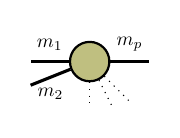
\begin{tikzpicture}[baseline=-0.5ex]
    \tikzset{tensor/.style = {minimum size = 0.5cm,shape = circle,thick,draw=black,inner sep = 0pt}, edge/.style = {thick,line width=.4mm},every loop/.style={}}
    \def\x{6}
    \node[tensor,fill=green!50!red!50!white] (A) at (\x,0) {$\At$};
    \draw[edge] (A) -- (\x-0.75,0) node [midway,above] {\scalebox{0.7}{\dimcolor{$m_1$}}};
    \draw[edge] (A) -- (\x+0.75,0) node [midway,above] {\scalebox{0.7}{\dimcolor{$m_p$}}};;
    \draw[edge] (A) -- (\x-0.75,-0.3) node [midway, below] {\scalebox{0.7}{\dimcolor{$m_2$}}};;
    \draw[dotted] (A) -- (\x,-0.6);
    \draw[dotted] (A) -- (\x+0.5,-0.5);
    \draw[dotted] (A) -- (\x+0.3,-0.6);
    \end{tikzpicture}
\hspace{0.3cm}
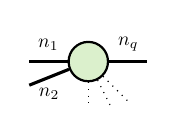
\begin{tikzpicture}[baseline=-0.5ex]
    \tikzset{tensor/.style = {minimum size = 0.5cm,shape = circle,thick,draw=black,inner sep = 0pt}, edge/.style = {thick,line width=.4mm},every loop/.style={}}
    \def\x{6}
    \def\y{0}
    \node[tensor,fill=green!70!red!20!white] (B) at (\x+1,\y) {$\Bt$};
    \draw[edge] (B) -- (\x+0.25,0) node [midway,above] {\scalebox{0.7}{\dimcolor{$n_1$}}};
    \draw[edge] (B) -- (\x+1.75,0) node [midway,above] {\scalebox{0.7}{\dimcolor{$n_q$}}};;
    \draw[edge] (B) -- (\x+0.25,-0.3) node [midway, below] {\scalebox{0.7}{\dimcolor{$n_2$}}};
    \draw[dotted] (B) -- (\x+1,-0.6);
    \draw[dotted] (B) -- (\x+1.5,-0.5);
    \draw[dotted] (B) -- (\x+1.3,-0.6);
\end{tikzpicture}\in\RR^{m_1\times\dots\times m_p\times n_1\times\dots\times n_q}.
$$
More generally, for any arbitrary number of tensors with arbitrary orders, the tensor network diagram of their outer product is obtained by simply placing them next to each other, e.g., for  $\Tt\in\RR^{d_1\times d_2\times d_3 \times d_4}$, $\Ab\in\RR^{m\times n}$ and $\vb\in\RR^{p}$
$$
\Ab\outprod \Tt\outprod \vb
=
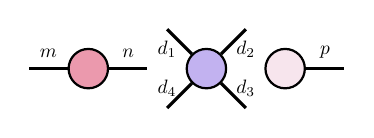
\begin{tikzpicture}[baseline=-0.5ex]
    \tikzset{tensor/.style = {minimum size = 0.5cm,shape = circle,thick,draw=black,inner sep = 0pt}, edge/.style = {thick,line width=.4mm},every loop/.style={}}
    \def\x{0}
    \def\y{0}
    \node[tensor,fill=blue!20!red!40!white] (A) at (\x,\y) {$\Ab$};
    \draw[edge] (A) -- (\x+0.75,\y)node [midway, above] {\scalebox{0.7}{\dimcolor{$n$}}};
    \draw[edge] (A) -- (\x-0.75,\y)node [midway, above] {\scalebox{0.7}{\dimcolor{$m$}}};
    \node[tensor,fill=red!20!blue!30!white] (T) at (\x+1.5,\y) {$\Tt$};
    \node[tensor,fill=red!70!blue!10!white] (v) at (\x+2.5,\y) {$\vb$};
    \draw[edge](T) -- (\x+2,\y-0.5);
    \node[draw=none] () at (\x+2,\y-0.25) {\scalebox{0.7}{\dimcolor{$d_3$}}};
    \draw[edge](T) -- (\x+2,\y+0.5);
    \node[draw=none] () at (\x+2,\y+0.25) {\scalebox{0.7}{\dimcolor{$d_2$}}};
    \draw[edge](T) -- (\x+1,\y-0.5);
    \node[draw=none] () at (\x+1,\y-0.25) {\scalebox{0.7}{\dimcolor{$d_4$}}};
    \draw[edge](T) -- (\x+1,\y+0.5);
    \node[draw=none] () at (\x+1,\y+0.25) {\scalebox{0.7}{\dimcolor{$d_1$}}};
    \draw[edge](v) -- (\x+3.25,\y)node [midway, above] {\scalebox{0.7}{\dimcolor{$p$}}};
\end{tikzpicture}\in\RR^{m\times n \times d_1\times d_2\times d_3 \times d_4\times p},
$$
is defined element-wise by $(\Ab\outprod\Tt\outprod \vb)_{i_1i_2j_1j_2j_3j_4k} = \Ab_{i_1i_2}\Tt_{j_1\cdots j_4}\vb_{k}$, where $i_1\in[m],i_2\in[n],j_l\in[d_l]$ for $l\in[4]$ and $k\in[p]$.

